\newcommand{\srroot}{Chapters/sr}

%%%%%%%%% TITLE
\section{Multi-frame face super-resolution}


\begin{abstract}

Face verification and recognition problems have seen rapid progress in recent years, however recognition from small size images remains a challenging task that is inherently intertwined with the task of face super-resolution. Tackling this problem using multiple frames is an attractive idea, yet requires solving the alignment problem that is also challenging for low-resolution faces. Here we present a holistic system for multi-frame recognition, alignment, and superresolution of faces. Our neural network architecture restores the central frame of each input sequence additionally taking into account a number of adjacent frames and making use of sub-pixel movements. We present our results using the popular dataset for video face recognition (YouTube Faces). We show a notable improvement of identification score compared to several baselines including the one based on single-image super-resolution.


\end{abstract}

% !TEX root = ../Thesis_main.tex
\chapter{Introduction}

%video surveillance+
%person re-id+
% originates from Multi-Target Multi-Camera Tracking 
%open world / closed world+
%face : verification/identification
%common aspects: detection , processing, recognition
%deep learning

%retrieval
%fine-grained recognition
%adaptation

%datasets (cut from the papers) + table with reid dataset?
%architectures
%definitions?
%contribution - what is done
\section{Context}
\subsection{Problem of 3D reconstruction}

\subsection{Approaches for solving 3D Reconstruction problem}

Solutions for a reconstruction problem can be grouped in two major groups: 1) Geometric approach - when problem is represented as optimisation of scene state given constrains on projections of scene state to data, 2) Machine Learning approach - inverse model is optimisation.

If $X$ - is scene data, $z$ - is the state of the scene, and $g_i(z)$ - projection function of 3D scene $z$ state to perspective $i$, then to find an optimal 3D reconstruction, one solves this minimisation problem:
\begin{equation}
z_{rec} = \min_z\sum_i|X_i-g_i(z)|_2 .
\end{equation}

This approach only solves problem for once scene and does not provide any semantic information about it, only basic geometric information. 
The second approach is more modern and better fitted for machine learning applications, because instead of optimizing state of the scene, it's optimizes a model that performs computation from input data to some semantic (intrinsic) parameters, and can be described as following optimisation procedure:
\begin{equation}
\min_\theta\sum_i|X_i-g_i(f_\theta(\pi))|_2,\ \ \pi=I_\theta(\{X_i\}_i),\ \ z=f_\theta(\pi),
\end{equation}
where $\pi$ - are scene parameters, $f_\theta(\pi)$ - is a generative model that generates 3D state $z$ and it's function is determined by tunable parameters $\theta$.

In reconstruction process information can be introduced in two possible ways: 1) input signal - data measured by some spatial sensor, 2) by adding a priori knowledge while training the Inverse model or by design choice of reconstruction algprithm. Between the two source exist a fundamental trade-off and detirmination of which is dominant can be quite difficult \cite{tatarchenko2019single}.


\subsection{Objectives and Motivations}

The goal of this work to improve methods of 3D reconstruction in holistic context using deep learning systems. For efficient applications such as robotics in human environments and mixed reality more advanced machine perception systems are needed. Human perception is a complex system with several properties not all of which are replicated in modern machine perception systems. From cognitive sciences it's known that ability to model environments is one of the most important for perception system, in area of computer vision this is known as an ability to perform \textit{3D reconstruction} of scenes and environments. To solve this problem in a general case requires application of machine learning.

In particular, the development of such holistic deep 3D reconstruction system includes several important tasks:

\begin{itemize}
􏰀    \item Capturing scenes, complete with colour and depth data of a sufficient quality,
    \item Recalling objects from large scale database of objects,
    \item Segmenting variety of most common elements from sensor data, such as household objects and architectural components,
    \item Detecting and reconstructing shape and pose of and human bodies.
\end{itemize}

Each of these sub-tasks constitutes a challenge in the context of human perception.

The presence of noise in sensor data (e.g., consumer grade depth cameras) is a serious problem for all downstream sub-tasks, low fidelity of this data causes a considerable compaunding performance drop.

\subsection{3D data representations}

We can describe a 3D object in multiple ways, and codification of it's properties has ramifications about capturing different information about objects and scenes, as well as kinds of models that can regenerate them or computational resources needed to process it.
Each representation has it's own pros and cons. We assume 3D information representation to be positive effective and usefull if it captures more relevant information with less storage requirement (compression), increases signal to noise ratio of data, captures shape and texture properties with minimum trade-off.

Here are some popular examples of 3D data representations:
\begin{enumerate}
	\item Multiple 2D projections - captures surface texture, highly redundant representation if images overlap, also vulnerable to optic illusions.
	\item Voxels - simple, most of the time can be sparse, represents rough volumetric properties vell but losses most of surface properties.
	\item Point Cloud - are sparse in a sense that they don't capture empty space, losing all surface properties besides color and estimated normals and most of volumetric properties.
	\item 2.5D (RGB-D) images are widespread because of cheap measurement devices, capture volumentric depth but succeptable to occlusion of bodies in a scene and records a lot of noise with actual signal.
\end{enumerate}



%Motivation: RGB-D scanning is here and we want to have a fine-grained understanding of the 3D captures
In the recent years, a wide variety of consumer-grade RGB-D sensors, such as the Intel Real Sense, Microsoft Kinect, depth-sensor enabled smartphones, enabled inexpensive and rapid RGB-D data acquisition. Increasing availability of large, labeled datasets (e.g.,~\cite{chang2017matterport3d,dai2017scannet})  made possible development of deep learning methods for 3D object classification and semantic segmentation. At the same time, acquired 3D data is often incomplete and noisy; while one can identify and segment the objects in the scene, reconstructing high-quality geometry of objects remains a challenging problem.  

An example of the new approach in recent work 
\cite{avetisyan2019scan2cad}, uses a large dataset of clean, labeled geometric shapes
\cite{chang2015shapenet}, for classification/segmentation associating the input point or voxel data with object labels from the dataset, along with adapting geometry to 3D data.  This approach ensures that the output geometry has high quality, and is robust with respect to noise and missing data in the input.  
At the same time, a ``flat'' classification/segmentation approach, with each object in the database corresponding to a separate label and matched to a subpart of the input data corresponding to the whole object, does not scale well as the number of classes grows and often runs into difficulties in the cases of extreme occlusion (only a relatively small part of an object is visible). 
Significant improvements can be achieved by considering object \emph{parts}, or more generally part hierarchies. 
Part-based segmentation of 3D datasets promises to offer a significant improvement both in finding the best matching shape in the dataset, recognizing objects from  highly incomplete data (e.g., from a couple of parts) from  as well as more precise geometry adaptation as well as, potentially, assembly of new shapes out of existing parts yielding a closer match to the input data. 

large collection of 3D models in database can be reduced to structured representations, 
objects with occluded sub-parts still can be recognized by parts available in the scan and the rest can be guessed with high probability, using parts, we can reconstruct new objects that are not yet present in the database of shapes.

Based on different approaches for volumetric information integration, from enhancements of  methods such as volumetric fusion \cite{curless1996volumetric}, to probabilistic  methods, and plethora of methods based on their combinations.

Compared to computer graphics models manually created by 3D professionals, 3D scans are noisy and incomplete.
Amount of noise and limited resolution of consumer-grade scanning hardware pose significant challenges for solving this important problem of scene reconstruction. 
Approaches of reconstruction based on fitting existing 3D assets into scene scans, have shown a lot of promise but still had problems with finding exact models from large database such as ShapeNet \cite{chang2015shapenet}, because of occlusion and lack of spatial context.

Learning-based approaches are very good at extracting features representative of objects and scenes as a whole, allowing to fill in occluded areas or guess parts affected by noise \cite{dai2017shape,dai2018scancomplete,song2017semantic}. These features are sufficient for scene completion, but they are not as good at recovering geometric primitives like: sharp edges, planar surfaces or borders between sub-parts, resulting in reconstruction quality much poorer than that of 3D content created by humans.

In this work, we focus on the key problem of semantic part segmentation of objects in the scenes, enabling further improvements in  dataset-based reconstruction. 
Semantic part-segmentation, can help in these situations, when sufficient number of the object parts is visible model can infer the non-visible parts essentially completing an object in sense of maximum probability conditioned on input data.

In human-made environments, a lot of objects have naturally defined semantic sub-parts, and those sub-parts can, in turn, have their sub-parts, i.e., parts form \emph{hierarchies}.  In our work, we use scene and object representation based on such part hierarchies.  We show how a part-labeled dataset of scanned 3D data suitable for machine learning applications can be constructed, and used to improve the performance of segmentation algorithms. 

Definitions of sub-parts are based on a set of primitive elements that were manufactured by one formation method or from one material.

Because of that and the fact that static scenes have other relationships between objects (fixed to each other or in direct surface contact), it's reasonable to suggest a scene description format that possesses a property of hierarchy (e.g., trees or other kinds of graphs).
Representing scenes as a discrete structures with multiple relationships between nodes. Such relationships like composability of its parts and affordances between whole objects, in turn allowing to compose a scene from separate objects.

\todo{merge these paragraphs}

In domain of human-made environments a lot of objects have sub-parts and those sub-parts can in turn have their own sub-parts. Definition of sub-part is often based on a set of primitive elements that were manufactured by one formation method or from one material. Because of that and the fact that static scenes have other relationships between objects (fixed to each other or in direct surface contact), it's reasonable to suggest a scene description format that possess a property of hierarchy (e.g. trees or other subgraphs).
A lot of researchers over the last 20 years came to the same conclusion. A lot of work on that problem was done by Mumford and Zhu in \cite{zhu2006stochastic}.

One of the papers dealt with problem of modeling Images as a hierarchy of super-pixels. \cite{russell2009associative}, or as a tree of geometric primitives (e.g. cylinders, spheres or 3D boxes) \cite{li2017grass}.

% point cloud (PC) turned in to a graph (based on proximity) point-cloud parser network reduces number of nodes and edges and enriches their feature vectors. First part of the decoder network functions similar to Feature Pyramid Network in CNNs, which performs local computations on different scales, followed by "pooling or convolutions" with reduced spatial component and increased feature components, thus leaving only small number of "keypoints" required to outline shapes of objects.



CAD constructor network translates that graph into CAD object (tree with primitives and combination rules). CAD rendered makes a mesh out of that object thus a residual between original PC and Mesh can be calculated.

Proximity Graphs - concept that allows to build a bridge between Point Clouds and Graph Processing. This area of computational geometry has a lot of theoretical results to offer for Deep Learning piplene designer.


\subsection{Definitions and examples}
\subsection{Data sources and devices}

\section{Inverse Graphics Problem formulation}

\cite{rezende2016unsupervised,eslami2016attend,kulkarni2015deep,wu20153d,izadinia2017im2cad}

Inverse graphics approach enables to solve a problem of "real-world" scene understanding through reconstruction of that scene and comparison it to measured data in some form.

Because it's a fairly new method it has some unexplored facets:
\begin{enumerate}
    \item How can we scale to hundreds and thousands of objects with different parameters.
    \item Embedded representations better than procedural generation
    \item Are there format that can have all advantages of CAD models and probabilistic properties that arise from real-world uncertainties.
\end{enumerate}

Central goals of computational perception is to get structured description of scenes from measurements such as photographic images, scans and videos.

Computer Vision as Inverse Graphics is the most rational formulations that could help us achieve this goal.

In the past, it has been hard to directly solve these problems in practice because of computational limitations.

However, it may be right time to take another look at this idea due to significant advances in deep learning for computer vision, probabilistic programming, and computer graphics.

Probabilistic programming - a tool that allows us to implement complex models while keeping ability to perform inference, extend with other probabilistic models by being general-purpose.

Re-formalizing inverse graphics in terms of probabilistic programming and deep learning allow us to solve even more complicated vision problems with off-the-shelf computational technology.

To make this approach scalable, my research can incorporate effective techniques such as: approximate Bayesian computation, differentiable programming for rendering.

Computer Graphics nowadays seems to be improving at a great pace in terms of designing solutions for hard image synthesis problems, but these solutions are usually hand-made and not flexible enough to cover all needs for general-purpose real world object generating, latest advances in generative models can help with that.


\subsection{Overcoming lack of information}

\section{Datasets}

Only recently research community started accumuulating sugnifficant amount of algined sensor data to solve large scale 3D reconstruction problems in deep learning context. In last 4 years we saw an explosion of 3D shape databases and 2D-to-3D indoor scene datasets, such as ShapeNet, 2D-3D Semantic, Scannet and Matterport3D datasets. Because accuracy and reacall properties of deep learning models scale with amount and variety of data, number of state-of-the-art models grew as well.

\section{Architectures}

PanopticFusion~\cite{narita2019panopticfusion} is a model that is able to segment large indoor scenes and separate \textit{Stuff} and \textit{Things}.


For outdoor datasets Point Cloud representation of data is more common because of large empty spaces and the way LiDAR sensor collects data. In such setting instance segmentation is nessesary first step for reconstruction~\cite{zhang2020instance}.

\subsection{Multi-view models}

Detailed comparision of multi-view 2D CNN model and 3D volumetric CNN can be found in \cite{qi2016volumetric}.

\subsection{Implicit 2D models}

Like inverse graphics network. Model takes 2D images and returns 2D images with 3D properties changed. 

\subsection{3D convolutional models}

Model generates or processes voxel image with 3D convolutional operation implemented Dense or Sparse.

Semantic information can boost the reconstruction performance because deep learning systems are able to pick up onto consistent signal \cite{jiao2018look,tatarchenko2019single,kendall2018multi}.

\subsection{2D to 3D Projection models}

Model uses camera parameters to compute 3D representation using 2D/2.5D images and projection operation.

\subsection{Point Set layers}

Neural Network processes a set of points to classify, segment or predict new set of points.

\subsection{Graph-Convolutional layers}

Model processes Geometric Graph where nodes represent points registered on a surface of objects or parts of objects, and has geometric or other information representing edges between points. Layers process activations associated with nodes taking into account the connectivity.

\subsection{Differentiable rendering layers}

Rendering operation is implemented in a differentiable way, allowing backpropogation of gradient information from 2D images to meshes and textures of the objects being rendered.

\subsection{Mesh generating layers}

Neaural Network layers that can create a mesh by way of processing a template 3D shape with parametracised operation or meshing other 3D shape representation generated by computation from weights and input.

\subsection{Implicit 3D models}

Models like NeRF, PIFU3D, neural network implements a rendering function depending on view angle and other graphics parameters, one model represents one scene and don't generalise for viriety of scene inputs.



\section{Contributions}

% \chapt{hist}, \chapt{bilinear} and \chapt{gradrev} use  person re-identification architecture of \citep{Yi14} as a baseline method (it is also  described in \sect{intro_architectures}).  \chapt{bilinear} is based on the results of \chapt{hist}: the loss function introduced in \chapt{hist} is used for 
% all the experiments in \chapt{bilinear} as it was demonstrated to show the best performance for person re-identification. 
% The results of \chapt{gradrev} were chronologically the earliest among all the results presented in this work, therefore  methods  from \chapt{hist} and \chapt{bilinear} were not used there. 
% Although the contributions of each of the chapters are independent, they are all parts of building a person re-identification pipeline and can be applied simultaneously. 
% \chapt{wildface} considers domain adaptation for surveillance face recognition and uses the method from \chapt{gradrev} as one of the baselines.
 


\section{Related work}
\label{sect:related}

There are two main research directions dedicated to face recognition for low-quality data: (i) the face restoration approach and (ii) the domain adaptation approach. In the face restoration-based approach, low-quality images are enhanced and restored to facilitate recognition. The ability to reuse existing recognition systems that were developed for high-quality data comes as a natural benefit of such methods. Domain adaptation methods are conversely aimed to change the existing recognition systems so that they are better suited for the target domain (i.e.\ low resolution/quality images). We now provide a brief review of both approaches.

\subsection{Face restoration methods}

There is a vast range of methods that perform face restoration. In most of them, different degradation types are considered separately. Pan \textit{et al.} \cite{pan2014deblurring} propose an effective face deblurring method based on approximating blur kernel followed by non-blind deconvolution. The blur kernel  approximation is guided by the known non-blurred exemplar with the structure similar to the input image structure. 

In Zhang \textit{et al.}~\cite{ZhangYZNH11}, deblurring and recognition tasks are considered simultaneously. They use a sparse representation of the input image in terms of the gallery image set. The blur kernel and representation coefficients are estimated iteratively. Classification is finally performed based on the classes with the highest coefficients in the sparse representation.  


A number of recent methods \cite{TuzelTH16,ZhuLLT16,xu2017learning,huang2017wavelet} explore the task of restoration of extremely low-resolution images using deep neural networks. All these works utilize the paired (aligned) learning scheme, where the high-resolution ground truth is known for every low-resolution image in the training set. The low-resolution training data are simulated using synthetic degradation of the initial high-resolution images. In \cite{xu2017learning} and \cite{TuzelTH16}, a generative adversarial network~(GAN)~\cite{goodfellow2014generative} is used to force the restoration network to produce more natural images. In \cite{huang2017wavelet}, an additional structure-based loss that uses wavelet transform is suggested for the same goal. While the results of these methods are impressive, there is no direct way to use the paired learning approaches for the arbitrary combination of degradation factors that one may encounter when analyzing real images captured by surveillance cameras. 

\subsection{Domain adaptation methods}

Several recent works are dedicated to domain adaptation in the context of different recognition tasks \cite{Volpi_2018_CVPR,Hong_2018_CVPR,Deng_2018_CVPR,Bousmalis_2017_CVPR,Murez_2018_CVPR}. In \cite{Murez_2018_CVPR}, 
\cite{Bousmalis_2017_CVPR} and \cite{Deng_2018_CVPR}, image-level domain adaptation is performed for segmentation, classification and similarity learning (person re-identification) correspondingly. Hong \textit{et al.} \cite{Hong_2018_CVPR} and Volpi \textit{et al.} \cite{Volpi_2018_CVPR} resort to feature-level domain adaptation for segmentation and classfication tasks. Both feature-level and image-level techniques are used in \cite{Hoffman17}.

Some of the aforementioned methods \cite{Hoffman17,Deng_2018_CVPR,Murez_2018_CVPR} employ CycleGAN framework  to change the domain of training data for classification, segmentation, and person re-identification. Here we explore a similar approach for the task of face recognition in the presence of complex degradation factors.

Hong \textit{et al.} \cite{HongIRY17} and
Sohn \textit{et al.} \cite{SohnLZY0C17} approach face recognition tasks for low-quality image domain. They consider image degradation as a domain shift and perform feature-level unsupervised domain adaptation based on adversarial learning showing better recognition results. 
The works \cite{HongIRY17} and \cite{SohnLZY0C17} are very related to ours: the authors show that domain-specific data augmentation is essential for training face recognition systems. 
 However, in both works, the data augmentation is performed 'by hand' (the degradation types and hyper-parameters for transforms are chosen and fixed), while we augment the training data in an automatic manner utilizing the CycleGAN framework, which can also be viewed as an image-level domain adaptation.
%Additionally, in contrast to \cite{HongIRY17}, we do not consider extremely large pose variation. Instead, we are more focused on the image degradation factors (e.g. the combination of small size, blur, JPEG-compression). 
Differently from \cite{SohnLZY0C17}, where evaluation is performed for the Youtube faces dataset, we approach the task in the presence of the somewhat stronger domain shift, as our test data are captured by surveillance cameras and are mostly of much lower quality.




%Some works already successfully use CycleGAN technique to perform an unsupervised domain adaptation. \cite{CYCADA} approached semantic segmentation. % add avput CYCADA

%recognition and reconstruction approaches
% Several existing works consider restoration and recognition problems jointly. In some works, authors apply the recognition-based priors to achieve better restoration results. \cite{TODO , Xu} 

% There are also approaches jointly performing explicit recognition and restoration
% In \cite{TODO Close  the  loop:  Jointblind  image  restoration  and  recognition  with sparse representation prior , Baker} The  proposed  approaches  perform  recognition  using  a  limited  number  of  gallery  images.   In parallel, they reconstruct the input image and classify it based on labels of the most relevant examples found in the train set.

 
% One of the baselines used in this work applies the similar scheme: CycleGAN framework is used to transfer the low-quality test data into the high-quality domain, the domain classifier serves as 'restoration' loss. We additionally introduce the recognition component into this scheme: another baseline is the same CycleGAN but with domain classifier based that is learned using features calculated with the pre-trained face recognition network.




\section{Evaluated approaches}
\label{sect:method}
\bigskip
\indent\textbf{Face recognition for the low-quality image domain}\\
%\subsubsection{Face recognition for the low-quality image domain}
\label{sect:strategies}
In this work we consider and compare two main approaches to face recognition for surveillance data: 1) restoration-based approach and 2) domain adaptation of existing face recognition neural networks. 

We consider two facial image domains: \begin{itemize}
\item domain $T: \{X^{T}_{i} \}_{i=0}^{N_T}$ that includes low-quality facial images $X^{T}_{i}$ captured using surveillance cameras. Usually, there are no identity labels provided, as assigning identity labels is quite challenging and may not even be feasible.
\item domain $S: \{(X^{S}_{i}, Y^{S}_{i})\}_{i=0}^{N_S}$ that includes facial images $X^{S}_{i}$ harvested from the Internet. These images are usually of higher quality and are taken in good lighting conditions. We assume that the data in this domain are supplied with identity labels $Y_i$.
\end{itemize}  

According to the available labeling, we can consider two different pipelines for building face recognition systems for surveillance data. The first option is the restoration-based approach when we use transform $F^{T \rightarrow S}: T \longrightarrow S$ as a face restoration method and then apply existing recognition neural network $R^{S}$ that is pre-trained on images from the domain $S$. The second option is to use the transform $F^{S \rightarrow T}: S \longrightarrow T$ to transfer the large collections of labeled training data to the target domain of surveillance images. In this scenario, we retrain the existing face recognition networks resulting in the new adapted model $R^{T}$.

More formally, we consider the following two pipelines for face recognition in the domain $T$.  We denote $d^{T}$ and $d^{S}$ the descriptors produced by the domain-specific face recognition models $R^{T}$ and $R^{S}$. These descriptors may be used e.g.\ to identify matching and non-matching faces based on the distances between them. 
 
$F^{T \rightarrow S}: T \longrightarrow S$ and $F^{S \rightarrow T}: B \longrightarrow A$ are the image-level domain transfer mappings. In the restoration-based approach, we train the recognition model $R^{S}$ using labeled data  $\{(X^{S}_{i}, Y^{S}_{i})\}$ where $X^{S}_{i} \subseteq B$. We then test the learned model by computing the descriptors $d^{S}$ after applying the network $F^{T \rightarrow S}$:  $d^{S} = R^{S}(X^{T\rightarrow S}) = R^{S}(F^{T \rightarrow S}(X^{T}))$

In the domain adaptation approach, we train the recognition network $R^{T}$ using labeled data $\{(X^{S \rightarrow T}_{i}, Y^{S}_{i})\}$, where the training examples $X^{S \rightarrow T }_{i} = F^{S \rightarrow T}(X^{S}_i)$, $X^{S}_i \subseteq S$ are obtained by transforming the high-quality images to the low-quality domain using the learned transformation $F^{S \rightarrow T}$. In this case, we apply the learned network directly to the low-quality images by computing and working with their descriptors $d^{T} = R^{T}(X^{T})$. The two approaches are compared below.


%image describing train and test time for both schemes
\bigskip
\indent\textbf{Learning domain transfer mappings}\\
%\subsubsection{Learning domain transfer mappings}
\label{sect:domain_transfer}
We use the CycleGAN approach~\citep{ZhuPIE17} to simultaneously learn the domain transfer mappings in both directions: $ F^{T \rightarrow S}: T  \longrightarrow S$ (restoration-based approach) and  $F^{S \rightarrow T}: S \longrightarrow T$ (domain adaptation approach). Here we describe the objective functions used for learning the domain transfer architecture.

We use the variant of CycleGAN similar to the one introduced in \citep{LiuNIPS2017} as we found it resulting in more stable and visually more plausible results for our task than the original framework \citep{ZhuPIE17}. Following \citep{LiuNIPS2017}, we decompose the domain transfer mappings into the compositions of encoders and generators: $F^{T \rightarrow S} = G^{S} \odot E^{T} $ and $F^{S \rightarrow T} = G^{T} \odot E^{S} $. Here, the encoders $E^{T}$ and $E^{S}$ transfer input images to the latent space, and generators $G^{S}$ and $G^{T}$ map the input latent codes to the domains $S$ and $T$.
 
For inputs $X^{T} \subseteq T $ and $X^{S} \subseteq S $ the results of their transfer to the opposite domain will be:
\begin{equation}
    X^{T \rightarrow S} = F^{T \rightarrow S}(X^{T}; \theta^{T}_F) = G^{S}(E^{T}(X^{T}))  
\end{equation}
\begin{equation}
    X^{S \rightarrow T} = F^{S \rightarrow T}(X^{S}; \theta^{S}_F) = G^{T}(E^{S}(X^{S}))
\end{equation}

The objective function used by the CycleGAN approach for learning is composed of the two symmetric parts:
\begin{equation}
\mathcal{L} = \mathcal{L}^{T} + \mathcal{L}^{S},
\end{equation} where $\mathcal{L}^{T}$ further decomposes as:
\begin{equation}\label{eq:domain_loss}
     \mathcal{L}^{T} = \mathcal{L}_{\text{GAN}}^T + \lambda_1 \mathcal{L}_{\text{cycle}}^T + \lambda_2 \mathcal{L}_{\text{rec}}^T,
\end{equation}
while $\mathcal{L}^{S}$ has same structure as $\mathcal{L}^{T}$:
\begin{equation}\label{eq:domain_loss2}
     \mathcal{L}^{S} = \mathcal{L}_{\text{GAN}}^S + \lambda_1 \mathcal{L}_{\text{cycle}}^S + \lambda_2 \mathcal{L}_{\text{rec}}^S,
\end{equation}


We now describe each of the terms in \eq{domain_loss}.
The GAN loss serves as the optimization objective for the domain transfer: 

\begin{dmath}
\mathcal{L}_{\text{GAN}}^A = 
    \min_{\theta^{S}_F} \max_{\theta^{T}_D} \mathbb{E}_{x \sim p_{X^{T}}} \log D^{T}(x) +
    \mathbb{E}_{x \sim p_{X^{S}}} \log \big(1 - D^{T}(F^{S \rightarrow T}(x)) \big)\,
\end{dmath}


Here, $D^{T}(X;\theta^{T}_D)$ and $D^{S}(X;\theta^{S}_D)$ are discriminators for the domains $T$ and $S$ that are trained in parallel with the training of the domain transforms.

The other two terms are the so-called cycle consistency loss: 
\begin{equation}
\mathcal{L}_{\text{cycle}}^T = L_1(F^{S \rightarrow T}(F^{T \rightarrow S}(X^{T})), X^{T})  
\end{equation}
and the reconstruction loss:
\begin{equation}
\mathcal{L}_{\text{rec}}^T = L_1(G^{T}(E^{T}(X^{T})), X^{T}) 
\end{equation}
In both terms, $L_1(\cdot,\cdot)$ denotes the $L_1$ distance.

We show the results of transferring the Internet and surveillance images to the other domain in figure \ref{fig:lr_hr_gan_res_ytube_initial_degraded}. While these results look interesting, we do not analyze their visual quality, as we are ultimately interested in the recognition performance rather than obtained visually-convincing images.

\bigskip
\indent\textbf{Learning face recognition models}\\
%\subsubsection{Learning face recognition models}
\label{sect:face_recognition}
In both scenarios that we compare in this paper, we need to train a face recognition model that turns images into vectorial descriptors. This happens either in domain $S$ (in the face restoration approach) or in domain $T$ (in the domain adaptation approach).

In either case, the goal of the training is to build a deep convolutional network that converts face images to the descriptors, such that matching face images have close descriptors and non-matching face descriptors have dissimilar descriptors. We use the Binomial Deviance loss~\citep{Yi14} to perform such training \eq{bindev}. We note that the choice of a particular metric learning loss is orthogonal to our study.

Alternatively to the models trained using the setting discussed above, we also consider reusing the VGG face model trained by the authors of~\citep{parkhi2015deep} on the VGG-face dataset.
\section{Experiments}
\label{sec:4}
\subsection{ModelNet40 dataset}
In our experiments we used well known data set of 3D objects ModelNet40.
It is a subset of 40 classes of larger data set called ModelNet \cite{wu20153d} that contains different 3D CAD models in OFF format.

The total size of ModelNet40 data set $12311$.
The data set is split into training and test subsets, their sizes are $9843$ and $2468$ correspondingly.
The data set is not balanced.
Number of samples per class vary: from 64 to 889, see Figure \ref{fig:modelnet_classes}.

\begin{figure}
	\centering
    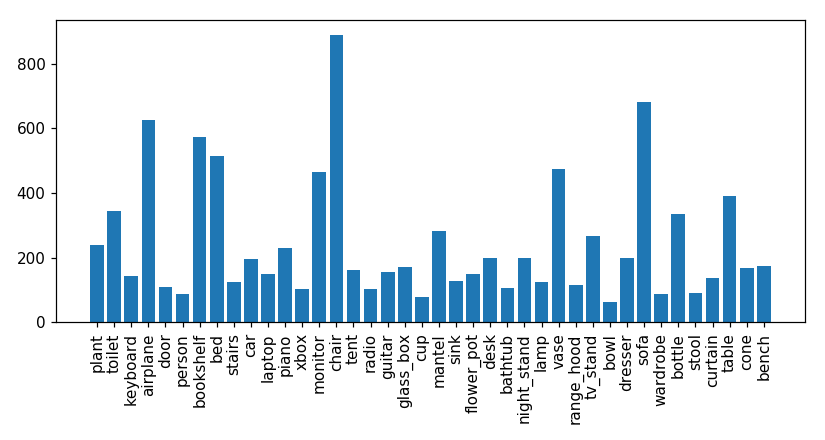
\includegraphics[width=\textwidth]{Figures/shape_retrieval/modelnet_classes.png}
    \caption{ModelNet40 data set: distribution of samples per class.}
    \label{fig:modelnet_classes}
\end{figure}

\subsection{Implementation details}
To demonstrate the impact that the triplet based training has on the performance of CNN descriptors
we use a deep network architecture shown in a Table~\ref{tab:net-architecture}. This network was implemented in PySparseConvNet, which is our modification of the SparseConvNet library \cite{graham2014spatially}. Besides new loss functions PySparseConvNet can be accessed from Python for a more interactive usage.

When forming a triplet for training we choose uniformly randomly a positive pair of objects from one class
and select a negative sample uniformly randomly from one of other classes.

For the optimization we use the SGD \cite{bottou-tricks-2012}, and the training is done
\begin{itemize}
\item in batches of size from $45$ to $90$ depending on a GPU video memory,
\item with a learning rate of $0.002$,
\item and a momentum equal to $0.99$.
\end{itemize}
Training can take up to a week on a server with advanced GPU, such as NVIDIA Titan X or GTX980ti.

\begin{figure}
\centering
\begin{tabular}{ccccc}
  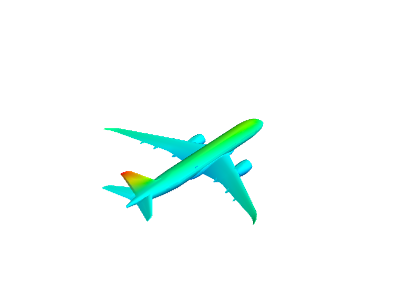
\includegraphics[width=0.19\columnwidth]{Figures/shape_retrieval/pic_airplane_solid.png} &
  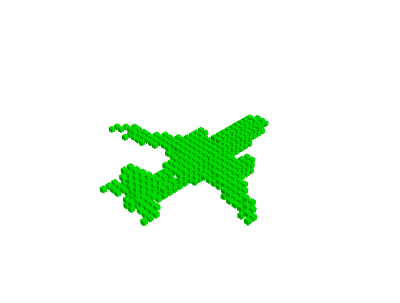
\includegraphics[width=0.19\columnwidth]{Figures/shape_retrieval/pic_airplane_30_solid.png} &
  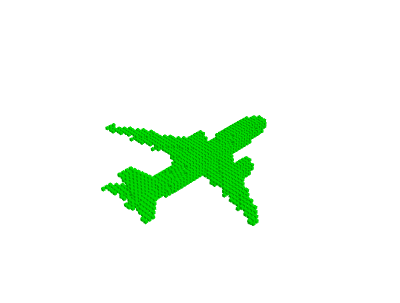
\includegraphics[width=0.19\columnwidth]{Figures/shape_retrieval/pic_airplane_50_solid.png} &
  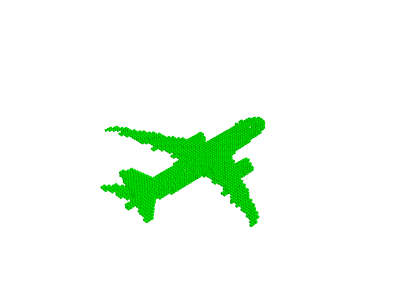
\includegraphics[width=0.19\columnwidth]{Figures/shape_retrieval/pic_airplane_70_solid.png} &
  
\includegraphics[width=0.19\columnwidth]{Figures/shape_retrieval/pic_airplane_100_solid.png} \\
% (a) first & (b) second \\
 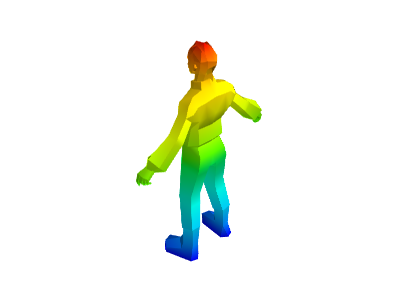
\includegraphics[width=0.19\columnwidth]{Figures/shape_retrieval/pic_person_solid.png} &
 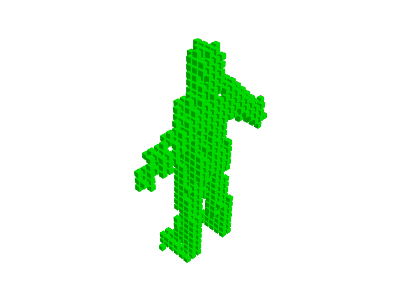
\includegraphics[width=0.19\columnwidth]{Figures/shape_retrieval/pic_person_30_solid.png} &
 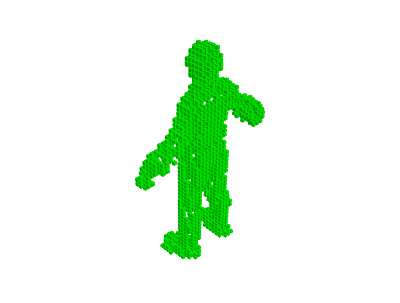
\includegraphics[width=0.19\columnwidth]{Figures/shape_retrieval/pic_person_50_solid.png} &
 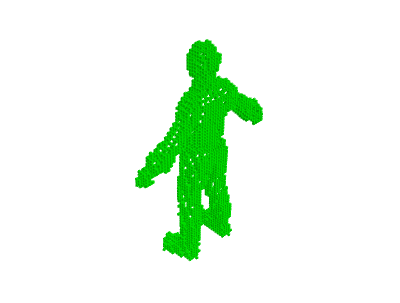
\includegraphics[width=0.19\columnwidth]{Figures/shape_retrieval/pic_person_70_solid.png} &
 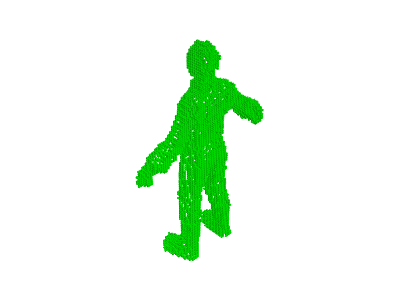
\includegraphics[width=0.19\columnwidth]{Figures/shape_retrieval/pic_person_100_solid.png} \\

 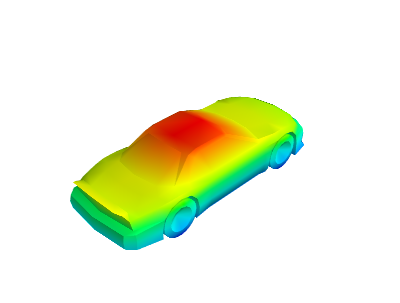
\includegraphics[width=0.19\columnwidth]{Figures/shape_retrieval/pic_car_solid.png} &
 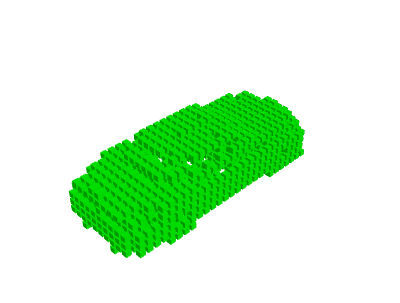
\includegraphics[width=0.19\columnwidth]{Figures/shape_retrieval/pic_car_30_solid.png} &
 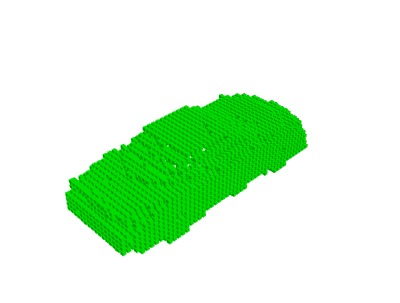
\includegraphics[width=0.19\columnwidth]{Figures/shape_retrieval/pic_car_50_solid.png} &
 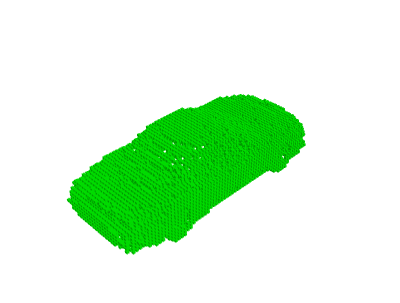
\includegraphics[width=0.19\columnwidth]{Figures/shape_retrieval/pic_car_70_solid.png} &
 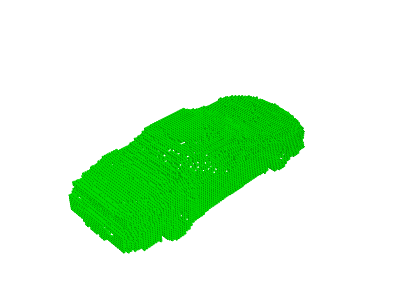
\includegraphics[width=0.19\columnwidth]{Figures/shape_retrieval/pic_car_100_solid.png} \\
\end{tabular}
\caption{Examples of some objects voxelizations at different resolutions $30$, $50$, $70$, $100$ (from left to right), left-most objects are depicted using original meshes}
\label{fig:voxels-examples}
\end{figure}


We train Sparse 3D Convolutional Neural Network (S3DCNN) on the 3D shape classification dataset by splitting it into  training and validation subsets, adding augmentation of data to achieve rotational and translational invariance. After training a model on a dataset of pairs, we use it to embed voxel representations of 3D meshes into $192$-dimensional space. The retrieval consist of ranking search objects by a cosine distance of vectors from a query vector.

The most popular metrics for evaluating retrieval performance are
\begin{itemize}
\item Precision-Recall Curve shows a trade-off between these two measures and how quickly the precision drops with the recall increase,
\item Mean average precision (mAP). Given a query, its average precision is the average of all precision values computed on all relevant objects in the retrieved list. Given several queries, the mean average precision (mAP) is the mean of average precisions for these queries. 
\end{itemize}
We evaluated mAP for different voxel rendering sizes of 3D shapes both at train and test times, see also Figure~\ref{fig:voxels-examples}.

To check if our model is comparable with other architectures, we consider a classification task. So, we trained our model for the classification task using the ModelNet40 train subset with 
\begin{itemize}
\item SoftMax last layer for $200$ epochs,
\item with exponentially discounting learning rate,
\item and performed retrieval evaluation on the test subset,
\item taking $20$ images from every class, and ranking them w.r.t their $L2$-norm by activations taken from the $17$-th layer.
\end{itemize}

Results of these experiments are provided in Table~\ref{tab:classification}. We can see that in case of classification task setup our model is comparable in terms of the classification accuracy, but mAP values are worse. But in case of metric learning performace of S3DCNN on mAP metric is much better.
Superior performance of retrieval task with MVCNN is not a surprising result, since MVCNN uses neural nets, pre-trained on ImageNet. On the other hand our model only requires 3D Shape dataset to learn.

In Figure~\ref{fig:map_for_rs} we provide the dependence of mAP on the input spatial resolution. We can see that the retrieval performance improves with increase in the input spatial resolution up to around $45-50$, after that it drops slightly and goes to plateau. It can be attributed to the insufficient amount of layers for the same scale of features, that can be separated in higher layers. Light blue color shows range of mAP on validation for top $30$ trained architectures.


\begin{figure}[!tbp]
\vspace{-20pt}
\centering
\begin{minipage}[b]{0.45\textwidth}
  \centering
  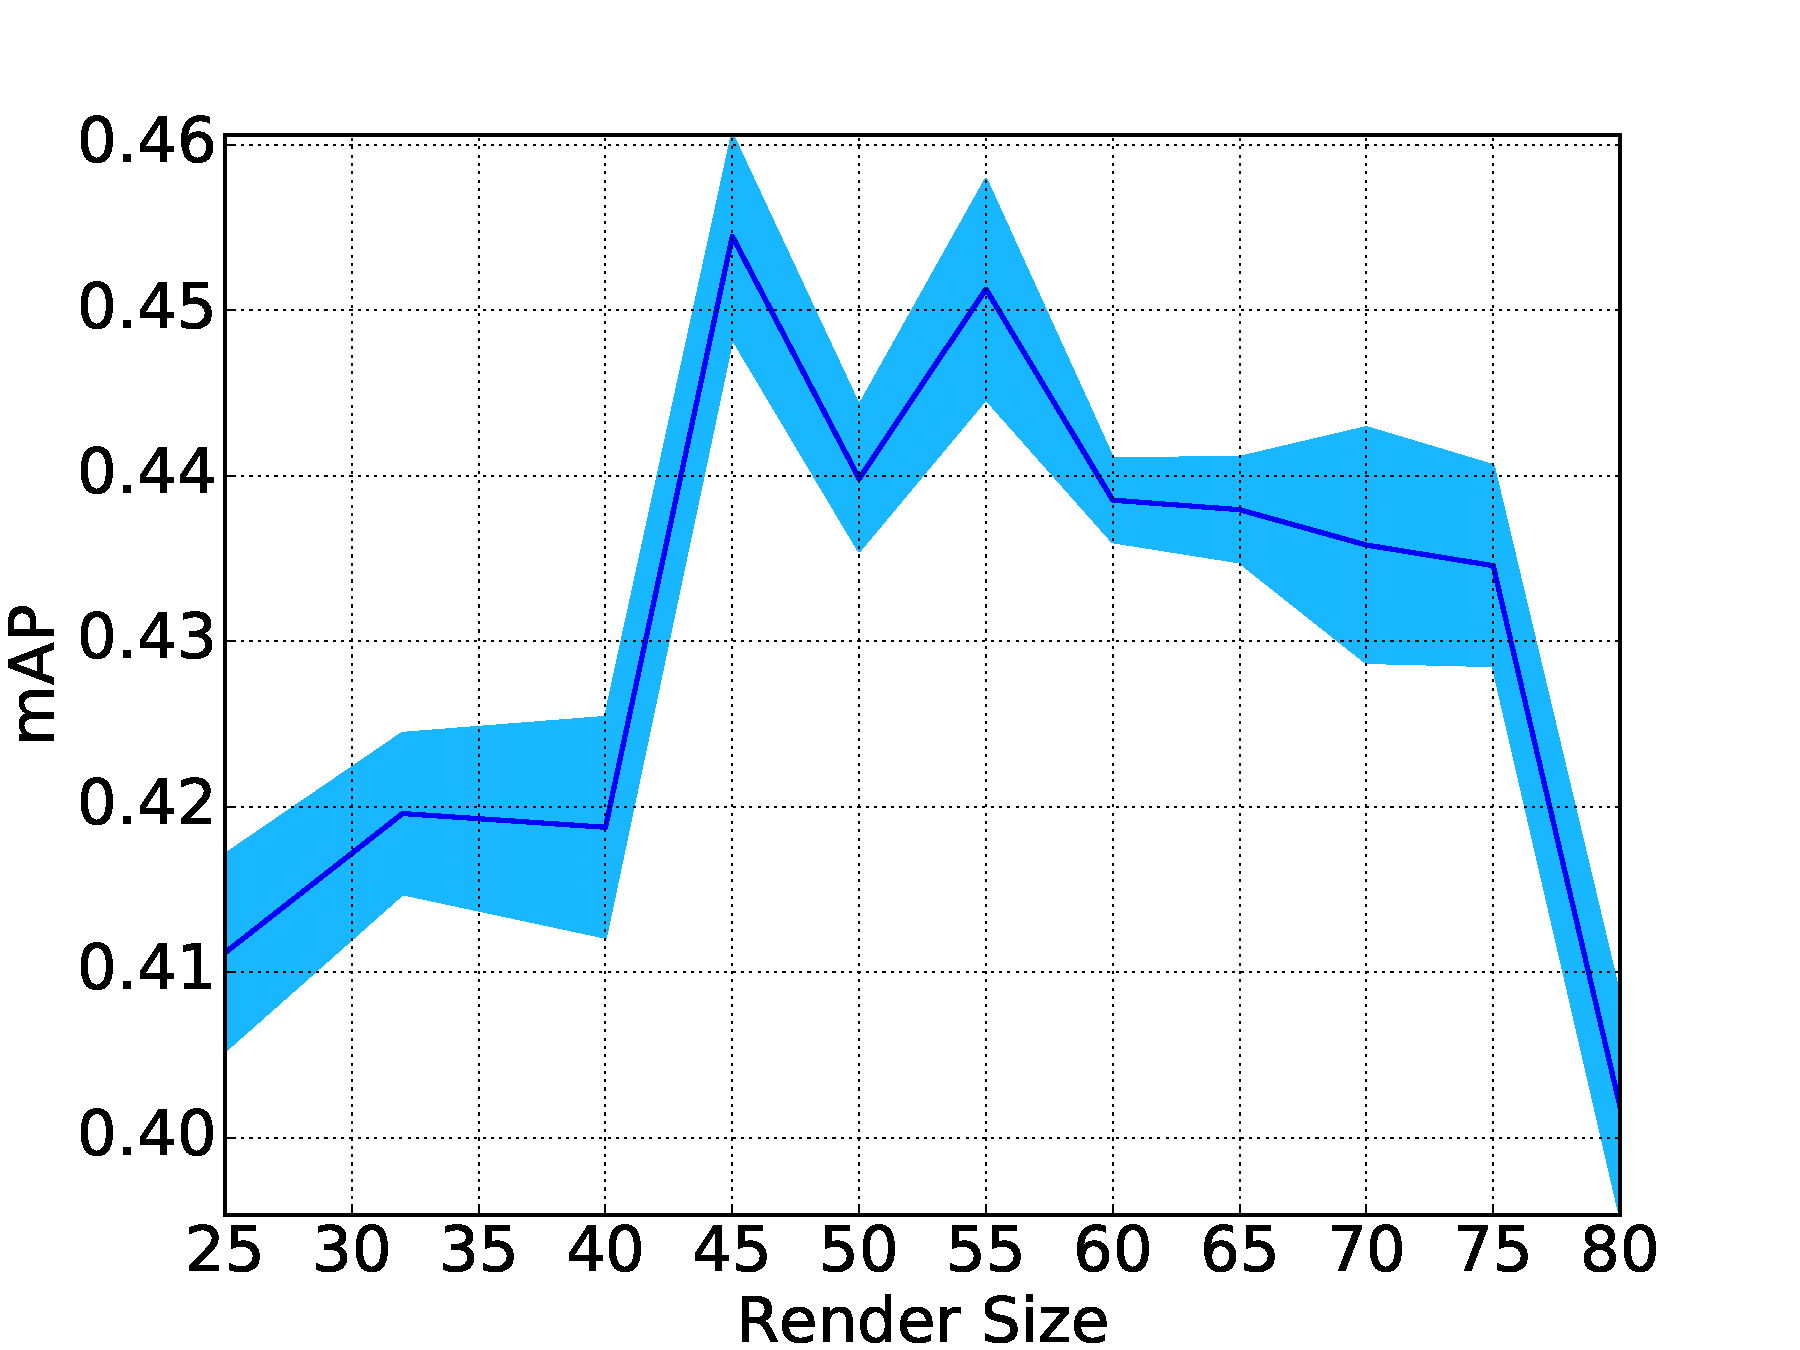
\includegraphics[width=\columnwidth]{Figures/shape_retrieval/new_map_to_rs.pdf}
  \caption{Dependence of the retrieval performance on the input spatial resolution}
  \label{fig:map_for_rs}
\end{minipage}
\begin{minipage}[b]{0.45\textwidth}
  \centering
  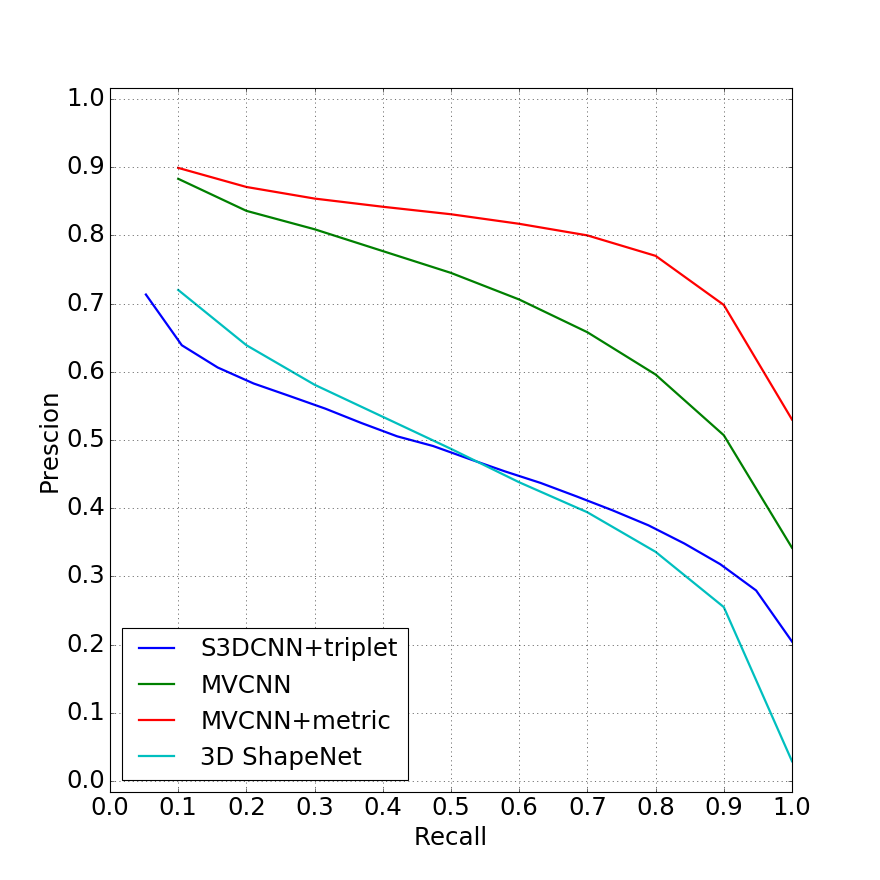
\includegraphics[width=\columnwidth]{Figures/shape_retrieval/pr_curves_comp}
  \caption{Precision-Recall curve for our method}
  \label{fig:pr_curve}
\end{minipage}
\end{figure}


We would like to note that in Figure~\ref{fig:map_for_rs} mAP values provided for different validation epochs and variability of best model can be explained by difference in total learning time.

% \begin{itemize}
% \item In Table~\ref{tab:classification} for the retrieval we used features from the last but one layer of the network,
% \item In Figure~\ref{fig:map_for_rs} we used learning with the triplet loss, for which we still have to better adjust the architecture and learning rate schedule.
% \end{itemize}


\section{Conclusion}
\label{sect:conclusion}

% Discuss your conclusions in order of most to least important.

In this chapter, we have compared the image-based domain adaptation techniques for face recognition in the presence of strong image degradation. We consider the recently proposed CycleGAN approach for learning mappings between the two domains of surveillance data and Internet face images. We demonstrate that the strategy of transferring the labeled Internet data to the surveillance domain and subsequent retraining the face recognition network helps to improve the recognition quality on real surveillance test data. We have investigated the variants of this approach, and have demonstrated that training on both transferred and original Internet data leads to the optimal performance. Finally, we show that in the case of our domain pair, the image-level adaptation approach outperforms feature-level domain adaptation. 

%Compare your results with those from other studies: Are they consistent? If not, discuss possible reasons for the difference.
We found our results consistent with \cite{SohnLZY0C17}, where face recognition for the low-quality is also considered. In \cite{SohnLZY0C17},  verification accuracy was improved using carefully chosen data augmentation. It is an interesting fact, that the improvement remained noticeable even when the data augmentation and the feature-level domain adaptation were applied simultaneously. Here, in contrast, we suggest performing the data augmentation in a more automatic way. Although we do not experiment with the combination of feature-level and image-level approaches to domain adaptation, we compare them independently. The combination of these adaptation techniques may further improve the results.


% Mention any inconclusive results and explain them as best you can. You may suggest additional experiments needed to clarify your results.
In our experiments, best results were achieved with training on both domains. An explanation can be given that the domain transfer model is imperfect and may push different images of the same identity too far as we do not use any kind of verification loss for training (ideally, this would require another pre-trained network for the low-quality domain, which essentially is the goal of this work). Therefore, keeping the initial data in the training set may result in less overfitting. %This can be explained by the fact that our target domain is not uniform in terms of data quality. We use two parts of the same track to generate matching pairs for each identity: e.g. these parts of each track differ in resolution (see \ref{fig:lr_hr_gan_res_ytube_initial_degraded}, columns $1$ and $3$). Therefore, using training data of diverse quality may lead to better results.  -- not true, checked.

% Briefly describe the limitations of your study to show reviewers and readers that you have considered your experiment’s weaknesses. Many researchers are hesitant to do this as they feel it highlights the weaknesses in their research to the editor and reviewer. However doing this actually makes a positive impression of your paper as it makes it clear that you have an in depth understanding of your topic and can think objectively of your research.

As an important negative result, we show that using CycleGAN-based restoration of lower-quality domain images by transferring them to the higher-quality domain does not bring consistent improvement to the recognition performance. We speculate that such transfer may distort some details of the images in a non-identity preserving way.

Our study considers a practically important domain of image data. 
We note, however, that our findings might not transfer to other pairs of domains in image adaptation.


% Discuss what your results may mean for researchers in the same field as you, researchers in other fields, and the general public. How could your findings be applied?
 
% State how your results extend the findings of previous studies.
% If your findings are preliminary, suggest future studies that need to be carried out.
% At the end of your Discussion and Conclusions sections, state your main conclusions once again.

